

\subsection{Data-Aware Declare Trace Alignment Pipeline}\label{sec:dadtap}
As per previous considerations, we want to show that it is sufficient to provide a specific characterization of $\Sigma$, which will be used to generate an automaton accepting symbols in $\Sigma$ and transforming traces as finite sequences in $\Sigma^*$. The proposed approach for obtaining $\Sigma$ from the Declare model $\varphi_{\mathcal{M}}$ is sketched in Figure~\ref{fig:twoexamples}, and described in detail in the following steps.

\begin{figure}[!t]
	%{\hspace{-1.3cm}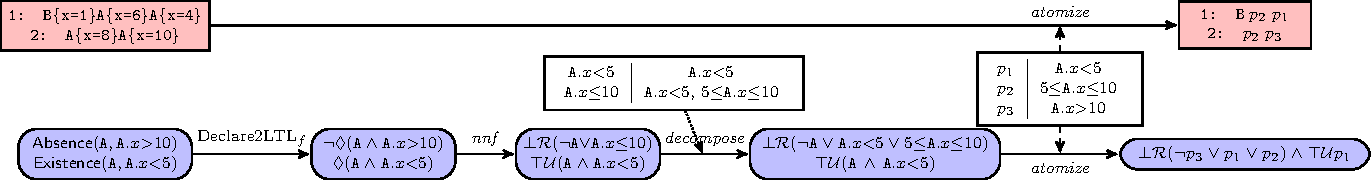
\includegraphics[width=1.3\textwidth]{images/example_1}}
	{\hspace{-1.3cm}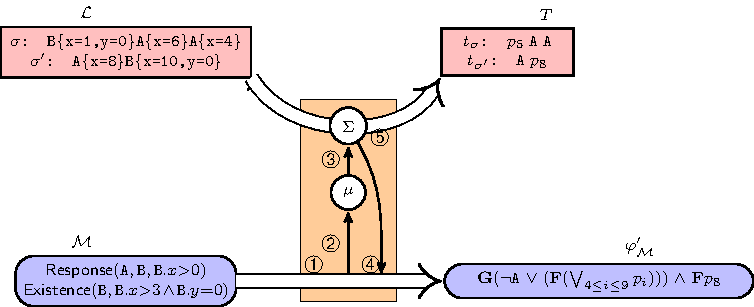
\includegraphics[width=1.3\textwidth]{images/example_3}}
	\caption{Intermediate steps required for obtaining $\Sigma=\Set{p_i|1\leq i\leq 9}\cup\{\texttt{A}\}$ from $\mathcal{M}$ and transforming $\mathcal{L}$ to a set of finite sequences, as well as generating an automaton from the resulting LTL$_f$ model (Figure~\ref{fig:g1g2}).}\label{fig:twoexamples}
\end{figure}
In step 1, we exploit the usual conversion of each single Declare clause into a LTL$_f$ formula in the \textit{negated normal form} \cite{LiPZVR20}, where negation is possibly pushed inside atoms ``$\texttt{a}.k\;\Re\; c$'' by replacing $\Re$ with its negation. 

In step 2, for each compound condition $\psi=\phi_{\texttt{a}}\wedge \phi^d$ over labels $\texttt{a}\in\textsf{Act}$, we collect all the atoms in $\phi_d$ in the form ``$\texttt{a}.k\;\Re\; c$'' for $k\in K$ in a map $\mu(\texttt{a},k)$. Contextually, we represent each atom as an interval, and we \textit{decompose} them
%
%%We now describe the main contribution of the paper, namely a technique for computing log trace alignments over Declare Data-Aware models. Our approach takes as input \begin{enumerate*}[label=\emph{\alph*})]
%	\item a Declare Data-Aware model $\mathcal{M}$ expressed as a set of instantiated templates,
%	\item a log trace $\sigma$,
%\end{enumerate*} and ranks the outcome of a LTL$_f$ conformance checking $\sigma\tilde{\vDash}\varphi$ accordingly to a data distance function $\mathcal{D}$.
%
%%The input transformation for reducing the data-aware alignment problem to the data-agnostic one is presented in Figure~\ref{fig:twoexamples} for two alignment examples. In particular, we first transform the Data-Aware Declare model, for then collecting the required information for providing the trace transformation.
%
%%\textbf{Data-Aware Declare Model Processing.} 
%
%
%
%
%%In step 3, we collect the data-aware predicates ``$\texttt{A}.\textit{var}\;\Re\;c$'' from all the model's clauses and group them by $\texttt{A}.\textit{var}$; each of these predicates is \textit{decomposed} 
into a disjunction maximal non-overlapping data-aware predicates. This task can be efficiently computed via interval trees \cite{inttree}. E.g., predicates $\texttt{B}.x>3$ and $\texttt{B}.x>0$ are first represented as intervals $\interval({3,+\infty})$ and $\interval({0,+\infty})$, and then decomposed into disjoint sub-invervals $\interval({-\infty,0}]$, $\interval[{0,3}]$, and $\interval({3,+\infty})$. Last, we replace the atoms in each LTL$_f$ formula by its decomposed representation, if any. 


In step 3, we put an atom $\texttt{a}\in\textsf{Act}$ in $\Sigma$ if the map $\mu(\texttt{a},k)$ is empty for each key $k\in K$; otherwise, given all the keys $k_{\texttt{a}_1},\dots,k_{\texttt{a}_h}\in K$ for which the map $\mu(\texttt{a},k_{\texttt{a}_i})$ is not empty, we partition the data space by combining the non-overlapping intervals as $\mu(\texttt{a},k_{\texttt{a}_1})\times\cdots\times\mu(\texttt{a},k_{\texttt{a}_h})$ obtained from the previous step. For each of this interval combination, we generate a fresh atom and put it in $\Sigma$. E.g., label \texttt{A} is never associated to a data condition, and therefore it will be associated to one single atom \texttt{A}. Concerning the label \texttt{B}, it is associated to data intervals over keys $x$ and $y$, which induce a space partitioning of 9 intervals, for which we generate distinct atoms $p_1\dots p_9$. As a result, we obtain $\Sigma=\Set{p_i|1\leq i\leq 9}\cup\Set{\texttt{A}}$.


%In step 4, for each event label \texttt{A}, we partition the data space \textit{var}$_1\times\dots\times$\textit{var}$_h$ associated to \texttt{A} by exploiting the disjoint intervals mined in the previous step. Each of such combination will be syntactically represented as a fresh \textit{atom}  proposition $p_i$: this implies that the label \texttt{A} is represented by the disjunction $\bigvee_ip_i$. When the data space associated to the predicates mined for \texttt{A} has only one property,  the atoms corresponds to the ones mined in the previous step. E.g., \texttt{A} in the first example from \ref{fig:twoexamples} is equivalent to $p_1\vee p_2\vee p_3$, and $\texttt{A}.\textit{x}<5$ is rewritten as $p_1$; given that such atoms represent disjoint intervals, then $\texttt{A}\wedge p_1\equiv p_1$. Similarly, $\neg \texttt{A}\vee \texttt{A}.\textit{x}<5\vee 5\leq\texttt{A}.\textit{x}\leq 10$ can be immediately rewritten as $\neg(p_1\vee p_2\vee p_3)\vee p_1\vee p_2$, which is equivalent to $\neg p_3\vee p_1\vee p_2$. Last, each LTL$_f$ representation of a Data-Aware Declare clause is represented into one single LTL$_f$ formula by conjunction and simplification.

Given the previously generated atoms, we can now generate a finite sequence for each log trace in $\Sigma^*$, and replace the propositions in the LTL$_f$ $\varphi_{\mathcal{M}}$ for $\mathcal{M}$ with a disjunction of atoms from $\Sigma$ as described in \S\ref{sec:wa}.
%
%\textbf{Data-Aware Log Trace Processing.} Given the atomization in Step 4, we process each data-enriched event within the trace as follows: if the event label is never associated with a data predicate, then we just discard the data information; otherwise, we replace each event with the single corresponding atom satisfying the associated semantics. Please observe that, by previous construction, each event can be represented by just one possible propositional atom, as the previous construction guarantees a partitioning (thus non-overlapping) representation of the data space.
E.g., all the trace events from Figure~\ref{fig:twoexamples} labelled as \texttt{A} are replaced with the atom \texttt{A}, as there are no data predicates in the model $\mathcal{M}$ that we can exploit to partition the data space. On the other hand, each data condition \texttt{B} is associated to a disjunction of atoms: event \texttt{B\{x=1,y=0\}} is uniquely represented by $p_5$, while event \texttt{B\{x=10,y=0\}} is uniquely represented by atom $p_8$. Similar considerations can be drawed for the $\psi$ predicate represented by the predicate $\mathcal{M}$: $\texttt{B}.x>0$ will be described by all the possible configurations of $y$ and data intervals $0<\texttt{B}.x\leq 3$ and $\texttt{B}.x>3$, which are identified by the disjunction $p_4\vee p_5\vee p_6\vee p_7\vee p_8\vee p_9$. On the other hand, $\texttt{B}.x>3\wedge \texttt{B}.y=0$ can be directly mapped to atom $p_8$.

\subsection{Automaton Manipulation for Trace Alignment}\label{ssec:amfta}

\texttt{\color{red}[TODO]} we consider insertions and deletions as possible repairs, while substitutions can be modeled by deletions followed by insertions. Synchronizations are \texttt{noops} requiring that a trace $\sigma$ at step $k$ contains a predicate $\phi$. 
\begin{itemize}
	\item synchronization $[\sigma_k\leftrightarrow \phi]$ aborts if $\sigma_k\neq\phi$, for  $1\leq k\leq |\sigma|$
	\item deletion\,\, $[\#\sigma_k\leftarrow \phi]::= \sigma_1\cdots\sigma_{k-1}\sigma_{k}\cdots \sigma_n$,\,\,\, for $n=|\sigma|$, $1\leq k\leq n$, and $\phi=\sigma_k$
	\item insertion $[@\sigma_k\leftarrow \phi]::= \sigma_1\cdots\sigma_{k-1}\phi\sigma_{k}\cdots \sigma_n$, for $n=|\sigma|$ and $1\leq k\leq n$
\end{itemize}
Therefore, any repair  of a trace $\sigma$ can be expressed in terms of a sequence of operations $\texttt{op}_1\cdots \texttt{op}_m$ which, when executed in appearance order, generate a novel trace $\tilde{\sigma}$ from $\sigma$.  \texttt{\color{red}[TODO]}


Last, the amount of repairs can be numerically quantified using a cost function $\mathcal{C}$ returning zero for any synchronization and $1$ otherwise; therefore $cost(\sigma, \tilde{\sigma})$ returns the minimal number of non-synchronization operations\footnote{Formally, $cost(\sigma,\tilde{\sigma})=\min_{\substack{\texttt{op}_1\cdots \texttt{op}_m,\\(\texttt{op}_m\,\circ \cdots\circ\, \texttt{op}_1)(\sigma)=\tilde{\sigma}}}\sum_{1\leq i\leq m}\mathcal{C}(\texttt{op}_m)$} required to obtain $\tilde{\sigma}$ from $\sigma$. Therefore, the conformance checking of a log trace $\sigma$ against a  Declare model represented as an LTL$_f$ formula $\varphi$ as in \cite{XuLZ17a} either returns $\sigma$ with cost zero if $\varphi\vDash\varsigma$ or, otherwise, returns a set of pairs $\Set{\braket{\tilde{\sigma},\texttt{op}_1\cdots\texttt{op}_m}_i}_{1\leq i\leq k, k\in\mathbb{N}}$, where\footnote{Formally, $\sigma\tilde{\vDash}\varphi = \Set{\braket{\tilde{\sigma},\texttt{op}_1\cdots\texttt{op}_m} | cost(\sigma,\tilde{\sigma}) = \min_\mu cost(\sigma,\mu),\;\tilde{\sigma}\vDash\varphi,\; (\texttt{op}_m\,\circ \cdots\circ\, \texttt{op}_1)(\sigma)=\tilde{\sigma}}$.} each trace $\tilde{\sigma}\in S$ is conformant to $\varphi$ and minimizes the alignment cost $cost(\sigma,\tilde{\sigma})$ via a repair sequence $\texttt{op}_1\cdots\texttt{op}_m$. We denote the output of such conformance checking as $\sigma\tilde{\vDash}\varphi$. 


\subsection{Encoding in PDDL}\label{ssec:eip}
\texttt{\color{red}[TODO]}